% Options for packages loaded elsewhere
\PassOptionsToPackage{unicode}{hyperref}
\PassOptionsToPackage{hyphens}{url}
\PassOptionsToPackage{dvipsnames,svgnames*,x11names*}{xcolor}
%
\documentclass[
  12pt,
]{article}
\usepackage{lmodern}
\usepackage{amssymb,amsmath}
\usepackage{ifxetex,ifluatex}
\ifnum 0\ifxetex 1\fi\ifluatex 1\fi=0 % if pdftex
  \usepackage[T1]{fontenc}
  \usepackage[utf8]{inputenc}
  \usepackage{textcomp} % provide euro and other symbols
\else % if luatex or xetex
  \usepackage{unicode-math}
  \defaultfontfeatures{Scale=MatchLowercase}
  \defaultfontfeatures[\rmfamily]{Ligatures=TeX,Scale=1}
\fi
% Use upquote if available, for straight quotes in verbatim environments
\IfFileExists{upquote.sty}{\usepackage{upquote}}{}
\IfFileExists{microtype.sty}{% use microtype if available
  \usepackage[]{microtype}
  \UseMicrotypeSet[protrusion]{basicmath} % disable protrusion for tt fonts
}{}
\makeatletter
\@ifundefined{KOMAClassName}{% if non-KOMA class
  \IfFileExists{parskip.sty}{%
    \usepackage{parskip}
  }{% else
    \setlength{\parindent}{0pt}
    \setlength{\parskip}{6pt plus 2pt minus 1pt}}
}{% if KOMA class
  \KOMAoptions{parskip=half}}
\makeatother
\usepackage{xcolor}
\IfFileExists{xurl.sty}{\usepackage{xurl}}{} % add URL line breaks if available
\IfFileExists{bookmark.sty}{\usepackage{bookmark}}{\usepackage{hyperref}}
\hypersetup{
  pdftitle={PS 813 Final Project},
  pdfauthor={Marko Kljajic \& Oliver Lang},
  colorlinks=true,
  linkcolor=Maroon,
  filecolor=Maroon,
  citecolor=black,
  urlcolor=blue,
  pdfcreator={LaTeX via pandoc}}
\urlstyle{same} % disable monospaced font for URLs
\usepackage[margin=1.25in]{geometry}
\usepackage{longtable,booktabs}
% Correct order of tables after \paragraph or \subparagraph
\usepackage{etoolbox}
\makeatletter
\patchcmd\longtable{\par}{\if@noskipsec\mbox{}\fi\par}{}{}
\makeatother
% Allow footnotes in longtable head/foot
\IfFileExists{footnotehyper.sty}{\usepackage{footnotehyper}}{\usepackage{footnote}}
\makesavenoteenv{longtable}
\usepackage{graphicx,grffile}
\makeatletter
\def\maxwidth{\ifdim\Gin@nat@width>\linewidth\linewidth\else\Gin@nat@width\fi}
\def\maxheight{\ifdim\Gin@nat@height>\textheight\textheight\else\Gin@nat@height\fi}
\makeatother
% Scale images if necessary, so that they will not overflow the page
% margins by default, and it is still possible to overwrite the defaults
% using explicit options in \includegraphics[width, height, ...]{}
\setkeys{Gin}{width=\maxwidth,height=\maxheight,keepaspectratio}
% Set default figure placement to htbp
\makeatletter
\def\fps@figure{htbp}
\makeatother
\setlength{\emergencystretch}{3em} % prevent overfull lines
\providecommand{\tightlist}{%
  \setlength{\itemsep}{0pt}\setlength{\parskip}{0pt}}
\setcounter{secnumdepth}{5}
\usepackage[scaled=0.875]{helvet} % ss \renewcommand{\ttdefault}{lmtt} %tt \usepackage{longtable} \usepackage{float}

\title{\textbf{PS 813 Final Project}}
\author{Marko Kljajic \& Oliver Lang}
\date{May 6 2020}

\begin{document}
\maketitle

\hypertarget{introduction}{%
\section{Introduction}\label{introduction}}

Over the past fifteen years, Mexico has experienced a surge in violence,
partly propelled by the state-coordinated militaristic crackdown on drug
trafficking and organized crime known as the ``War on Drugs''. Rising
violence has generated a nation-wide debate between the left (opponents
of militarization) and the right (supporters of militarization) on the
utility of using the military to combat drug trafficking. Critics of
militarization refer to well-documented cases implicating military
personnel in extrajudicial killings, enforced disappearances, torture,
sexual violence, and other rights abuses (HRW 2011; 2018). While a
majority of Mexicans are concerned about human rights violations,
military intervention continues to receive popular support from much of
the population (PEW 2012, 2017) partly due to mistrust in law
enforcement and the inability of police to uphold public security.
Supporters point to the popular demand for military intervention in
order to justify keeping the military in the streets until police reform
is successful.

However, popular demand for militarization is puzzling. Recent research
suggests that the militarization of anti-drug efforts has decreased the
state's capacity to provide public order and extract fiscal resources:
homicide and kidnapping rates have increased while tax collection has
decreased (Flores-Macías 2018). If popular demand for militarization
initially arose out of concern for personal security (Sotomayor 2013),
it is unclear why this support has continued. Contrary to expectations
of success, studies have shown that relying on the military for public
security has resulted in higher levels of violence (Espinosa \& Rubin
2015; Atuesta et al 2019) and other health-related issues (Aburto \&
Beltrán-Sánchez 2019; Michaelsen \& Salardi 2020) without addressing
organized crime in general (Shirk, Wallman, \& Osrio 2015) and drug
trafficking in particular (Lindo \& Padilla-Romo 2018). Given the
tension between positive expectations of military intervention for
public security and the negative consequences of intervention, what
strategies might exist to convey information about the negative effects
of militarization in a fashion that is more persuasive?

\hypertarget{theory}{%
\section{Theory}\label{theory}}

Issue framing is a technique that can be used to change the evaluation
of an policy issue by manipulating how it is presented and conveyed.
Framing has been shown to have a signficant effect on shaping public
attitudes across a range of policy issues (Jacoby 2000; Faricy \& Ellis
2014; Corner et al 2011; Boettcher \& Cobb 2006). On militarization in
Mexico, for example, Romero, Magaloni, and Diaz-Cayeros (2015) found
that pro-government framing of the success of military intervention
against drug trafficking enhanced support for this policy, but only
among individuals who did not experience drug-related victimization.

More recently, researchers have adapted insights from Moral Foundations
Theory, a social-psychological theory that explains the origins of and
variation in moral reasoning on politics and cultural issues (Graham et
al 2011), to explore the possibility of whether specially framed
political arguments, specifically those couched in the moral values of
the target audience, are better at moving public opinion than those that
are not. According to this theory, conservatives and liberals generally
endorse and rely on different moral values when making political
assessments and judgements. Liberals mainly focus on harm and fairness,
whereas conservatives tend to treat issues related to loyalty,
authority, and purity as more important (Haidt \& Graham 2007; Graham,
Haidt, \& Nosek 2009). These political differences help to explain many
of the disagreements between liberal and conservative judgements of
right and wrong (Haidt 2012) and diverging attitudes on many social
issues, including support for the military (Koleva et al 2012).

The most common framing technique used to lower support for using the
military against drug trafficking highlight how intervention has
increased violence and led to the violation of human rights. This frame
resonates with liberal audiences for whom such issues might be more
important because they violate notions of harm and fairness (Haidt \&
Graham 2007; Graham, Haidt, Nosek 2009). They might not resonate with
supporters of military intervention who might consider violence and
human rights violations as necessary byproducts of the ``War on Drugs''.
This might partly explain why there is both concern for human rights
violations but also steady support for militarization. Might another
frame be more effective? Military personnel have also been charged with
corruption and with cooperating with the very criminal organizations
they were ordered to neutralize (HRW 2011; 2018). Would framing the
consequences of military intervention in terms of collusion with cartels
(violation of loyalty), conspiracy (violation of authority), and
corruption (violation of purity) have a more powerful effect on
modifying popular support for militarization? We conduct a survey
experiment to test whether framing the outcomes of militarization in
terms of violations of loyalty, authority, and purity lower public
support for militarization compared to framing the issue in terms of
harm and fairness violations.

\hypertarget{data}{%
\section{Data}\label{data}}

We recruited a random sample of university students (n = 661, 301 Male,
357 Female, and 3 Other) from seven different universities in Mexico
during the winter of 2018. Participants were asked to complete a
comprehensive pre-treatment instrument that included basic demographic
information, experiences with drug-related victimization, various moral
beliefs about the role of government in Mexico, and political ideology.

Participants were then randomly presented with a newspaper article that
either frames the outcomes of a military intervention against drug
trafficking as violating harm/fairness norms (control) versus
loyalty/authority/purity norms (treatment).

\begin{longtable}[]{@{}ll@{}}
\toprule
\begin{minipage}[b]{0.47\columnwidth}\raggedright
Control\strut
\end{minipage} & \begin{minipage}[b]{0.47\columnwidth}\raggedright
Treatment\strut
\end{minipage}\tabularnewline
\midrule
\endhead
\begin{minipage}[t]{0.47\columnwidth}\raggedright
Last week, there were reports the Mexican military may have
\emph{violated human rights} in responding to a gun battle in which 11
people were killed. The Mexican office of the U.N. High Commission for
Human Rights said it obtained \emph{documentation of torture, poor
detention conditions and searches conducted without warrants} after the
intervention. Officers arrested at least 30 people after the shootout. A
representative of the commission, called for the investigation of all
deaths, \emph{including those that occurred during police proceedings}.
Mexico's military has been embroiled in multiple \emph{human rights}
scandals in recent decades, including \emph{extrajudicial killings of
gang members} and the disappearances of citizens. The non-partisan
commission will rule on these \emph{human rights allegations}\strut
\end{minipage} & \begin{minipage}[t]{0.47\columnwidth}\raggedright
Last week, there were reports the Mexican military may have
\emph{cooperated with local criminal organizations} in responding to a
gun battle in which 11 people were killed. The Mexican office of the
U.N. High Commission for Human Rights said it received \emph{reports of
collusion, conspiracy, and fabricated evidence}. Officers arrested at
least 30 people after the shootout. A representative of the commission
called for the investigation of all deaths and \emph{raised concerns
about containment of the armed forces by local criminal organizations}.
Mexico's military has been embroiled in multiple \emph{corruption}
scandals in recent decades, including \emph{working complicity with
gangs} in the disappearance of citizens. The non-partisan commission
will rule on these \emph{corruption allegations}.\strut
\end{minipage}\tabularnewline
\bottomrule
\end{longtable}

We used four dependent variables to evaluate the attitudes of
participants post-treatment. Our dependent variables are presented in
the table below. We measured participants' trust in the military from 1
(``Very Low Trust'') to 11 (``Very High Trust''); support for the army's
participation in the street and support for punishing soldiers involved
in the crimes reported on a 7-point Likert-scale from 1 (``Strongly
Disagree'') to 7 (``Strongly Agree''); and whether participants' would
change their opinion of the military if the report were to be confirmed
(0 - ``No'', 1 - ``Yes'').

\begin{longtable}[]{@{}ll@{}}
\toprule
\begin{minipage}[b]{0.29\columnwidth}\raggedright
Variable\strut
\end{minipage} & \begin{minipage}[b]{0.65\columnwidth}\raggedright
Outcome Text\strut
\end{minipage}\tabularnewline
\midrule
\endhead
\begin{minipage}[t]{0.29\columnwidth}\raggedright
Trust in army:\strut
\end{minipage} & \begin{minipage}[t]{0.65\columnwidth}\raggedright
To what extent do you trust the army?\strut
\end{minipage}\tabularnewline
\begin{minipage}[t]{0.29\columnwidth}\raggedright
Support for army participation:\strut
\end{minipage} & \begin{minipage}[t]{0.65\columnwidth}\raggedright
The army should keep participating in crime combat\strut
\end{minipage}\tabularnewline
\begin{minipage}[t]{0.29\columnwidth}\raggedright
Support for punishing soldiers:\strut
\end{minipage} & \begin{minipage}[t]{0.65\columnwidth}\raggedright
Soldiers that behave as mentioned by the experts should be severely
punished\strut
\end{minipage}\tabularnewline
\begin{minipage}[t]{0.29\columnwidth}\raggedright
Willingness to reconsider opnions:\strut
\end{minipage} & \begin{minipage}[t]{0.65\columnwidth}\raggedright
If expert concerns were real, would you reconsider your opinion about
the army?\strut
\end{minipage}\tabularnewline
\bottomrule
\end{longtable}

\begin{figure}
\centering
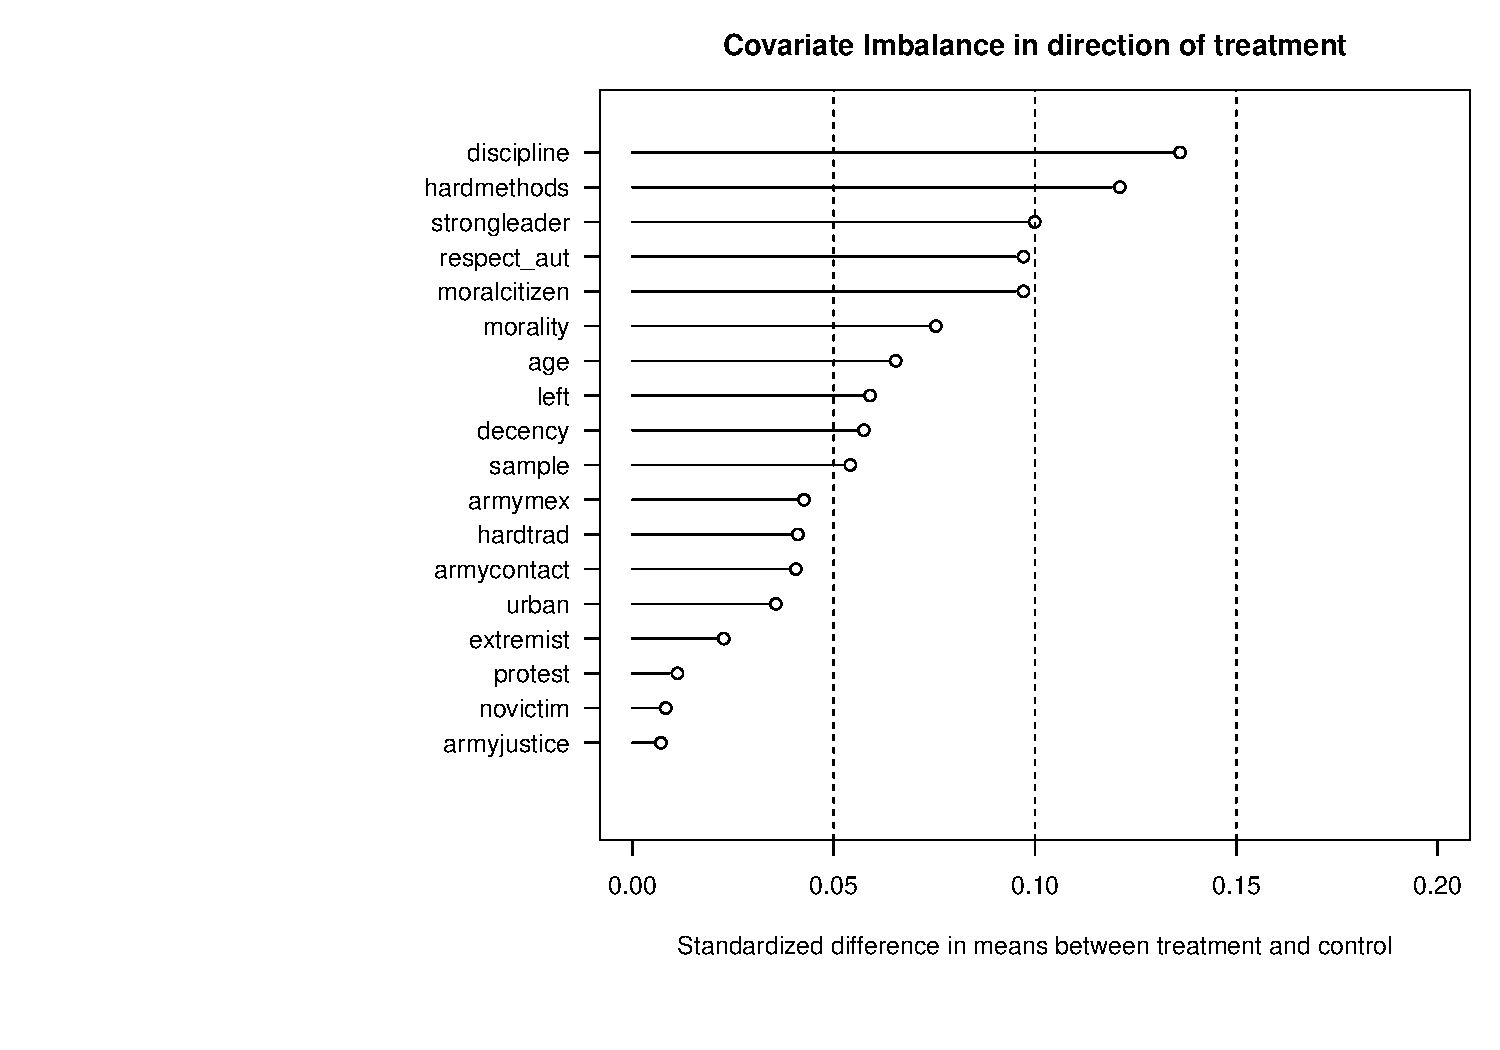
\includegraphics{marko-oliver_final-proj_files/figure-latex/unnamed-chunk-4-1.pdf}
\caption{Covariate Imbalance in direction of treatment}
\end{figure}

\begin{figure}
\centering
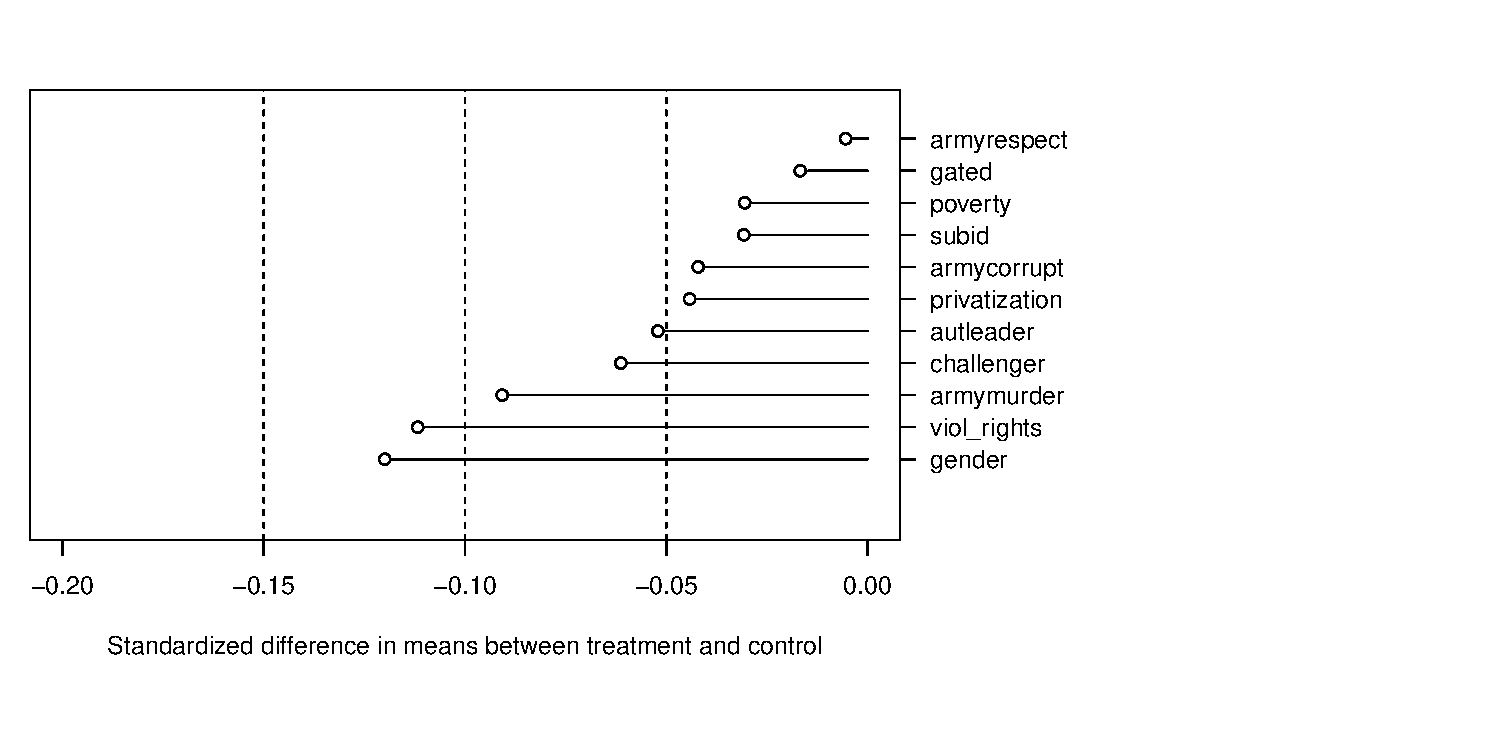
\includegraphics{marko-oliver_final-proj_files/figure-latex/unnamed-chunk-5-1.pdf}
\caption{Covariate Imbalance in direction of control}
\end{figure}

\hypertarget{estimation}{%
\section{Estimation}\label{estimation}}

We chose to estimate our effects in three ways. First, we used the
simple difference in means estimator. For our other two specifications,
we adjusted for pre-treatment covariates. The motivation for adjustment
was improving precision. We follow the procedure proposed by Lin (2013)
for regression adjustment in randomized experiments. Lin showed that
including centered pre-treatment covariates and their interactions with
the treatment in the model either equals or improves on the asymptotic
precision of the difference-in-means estimator. Additionally, the HC2
estsimator yields asymptotically valid confidence intervals. In contrast
with traditional regression adjustment, this property holds under less
stringent regularity conditions---neither linearity in the (our)
parameters nor homoskedasticity is necessary.

Since data is missing for some covariates, we estimated our models
twice. First, on data without any rows where covariates are missing,
which is the default in most packages. Second, on data where missing
observations are imputed using the imputation model proposed by Honaker
et al.~(2011). This method makes two assumptions. First that the joint
distribution of the observed and missing data is multivariate normal.
While we have many categorical variables in our data set whose values
are not going to be normally distributed, the Amelia package provided by
Honaker et al (2011). allows us to specify these variables which are
then rescaled during the imputation process. The second assumption is
that our observed data gives all the systematic information about
whether a given observation will be missing (MAR). While we cannot be
sure that this assumption is justified, the distribution of observed and
imputed observations looks similar for covariates where a larger
proportion of observations is missing (see appendix). While this does
not confirm that the imputation model is correct, there are at least no
glaring red flags that something is going wrong.

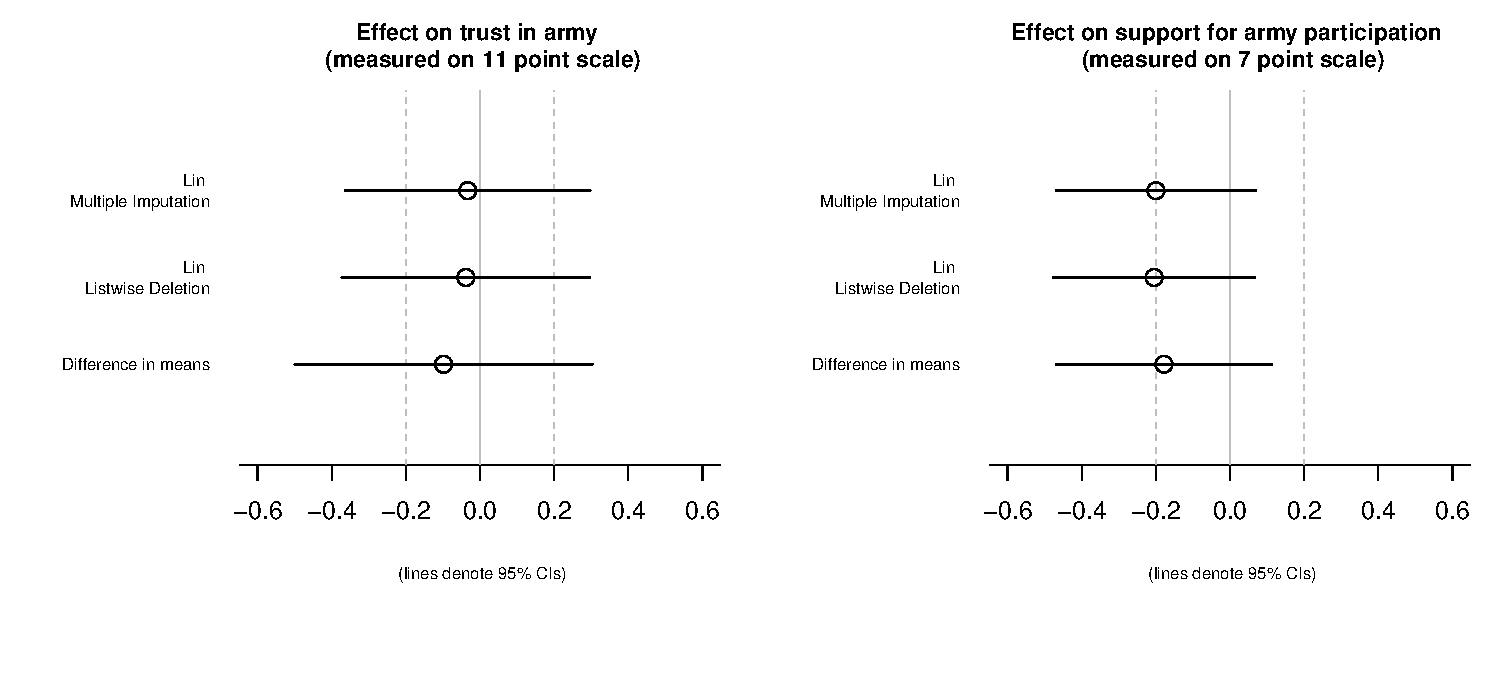
\includegraphics{marko-oliver_final-proj_files/figure-latex/unnamed-chunk-6-1.pdf}

\begin{figure}
\centering
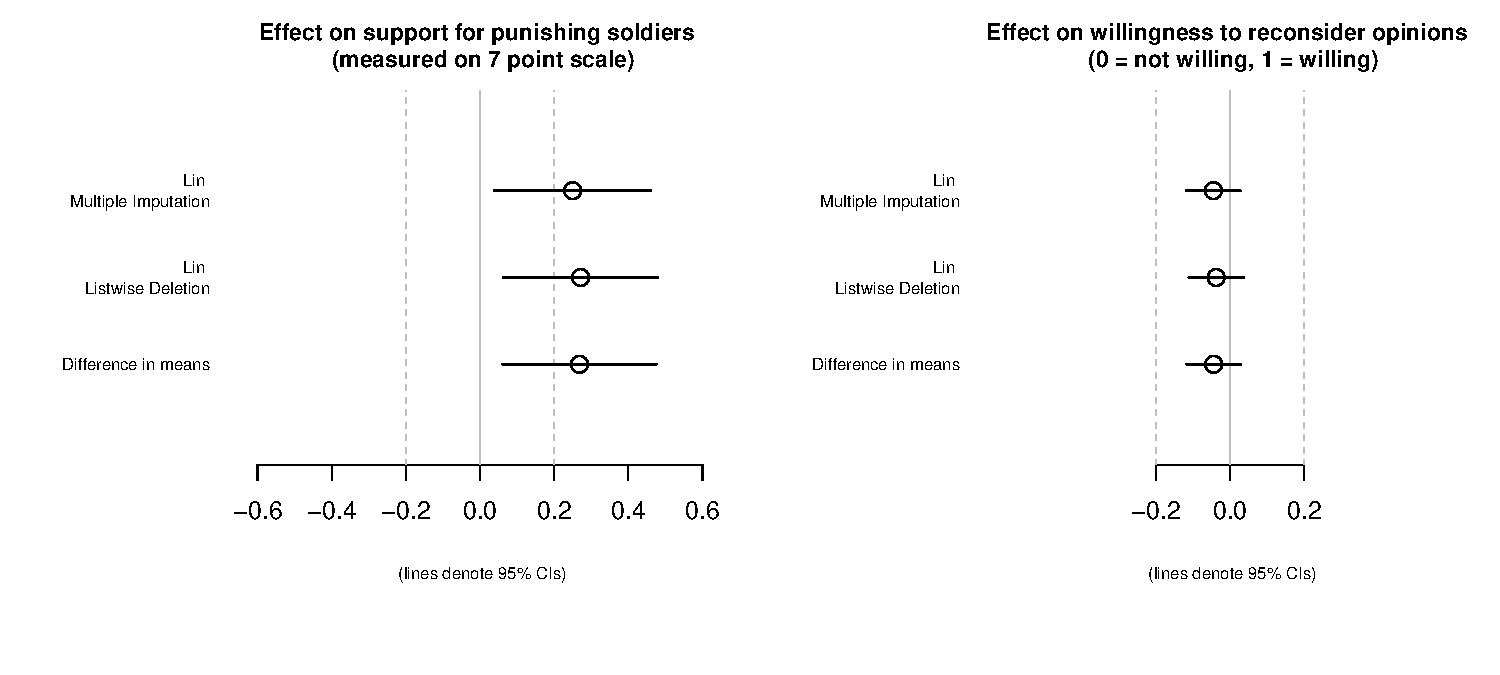
\includegraphics{marko-oliver_final-proj_files/figure-latex/unnamed-chunk-7-1.pdf}
\caption{Estimated treatment effects}
\end{figure}

\hypertarget{results}{%
\section{Results}\label{results}}

Figure three reports estimated treatment effects for each outcome. The
only treatment effect that we estimate wiith high levels of precision is
support for punishing soldiers. Across our three specifications, we
estimate that treatment with the loyalty / authority / purity issue
frame increases support for punishing soldiers on a 7-point scale by
0.25 (multiple imputation \& adjustment), 0.27 (list-wise deletion \&
adjustment), and 0.27 (difference-in-means). A 0.27 shift on the scale
is equivalent to 0.2 standard deviations. For each specification we
estimate that there is a greater than 95 percent chance that an interval
centered on the point estimates does not include zero.

Most of this effect is coming from shifts at the upper end of this
scale: esp.~a large increase in the proportion of respondents who were
extremely willing to punish soldiers. This is visible in the second line
of the below figure. For all other outcomes we do not estimate an
average treatment effect precisely and there seems to be few
diifferences in the overall distribution of answers.

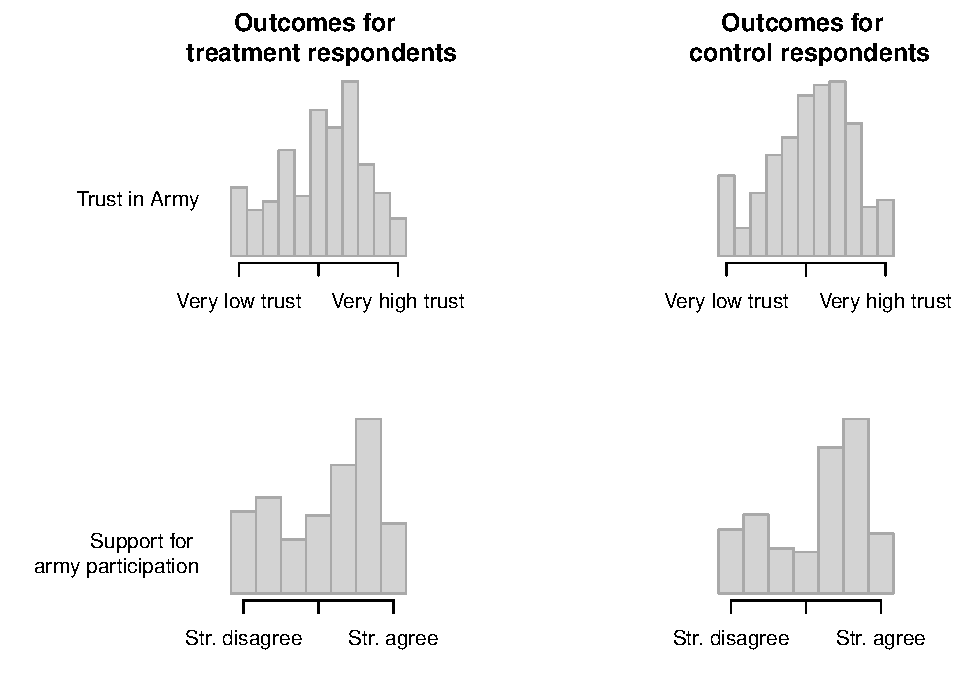
\includegraphics{marko-oliver_final-proj_files/figure-latex/unnamed-chunk-8-1.pdf}

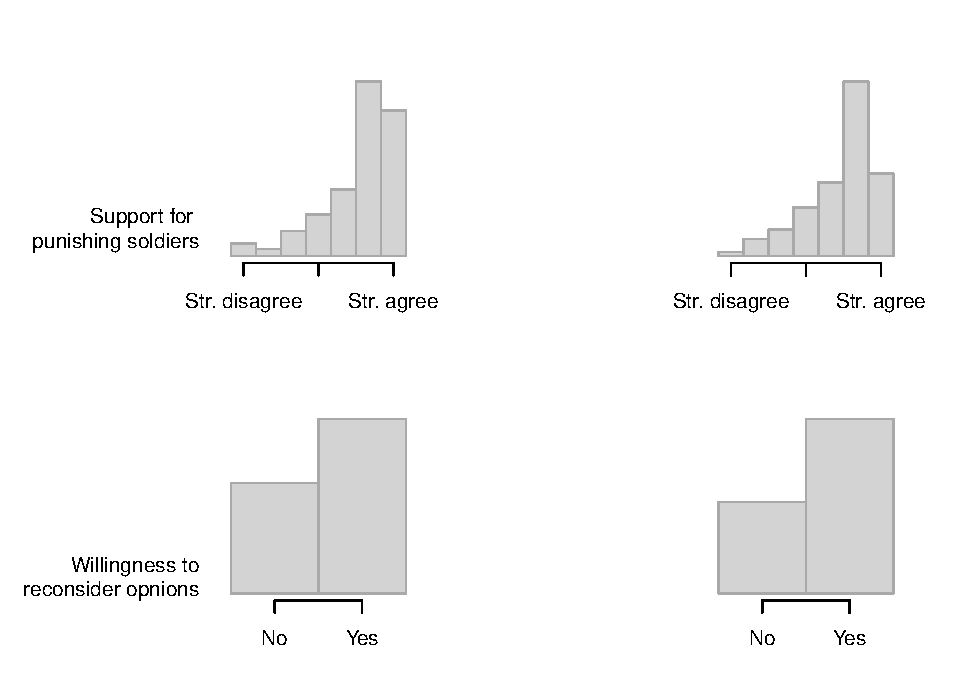
\includegraphics{marko-oliver_final-proj_files/figure-latex/unnamed-chunk-9-1.pdf}

\hypertarget{conclusion}{%
\section{Conclusion:}\label{conclusion}}

This study sought to test whether framing the consequences of military
intervention in terms of corruption and conspiracy rather than human
rights violations was more effective in modifying public support for
militarization. We found that the framing condition did not have a
statistically significant effect on trust in the military, support for
army participation in combating drug trafficking, and willingness to
change one's opinion about the issue, but they were in the predict
direction. However, we did find a significant effect in the predicted
direction (positive) for support for punishing soldiers who comitted the
crimes in the treatment.

\hypertarget{work-cited}{%
\section{Work Cited}\label{work-cited}}

Aburto, José Manuel, and Hiram Beltrán-Sánchez. 2019. ``Upsurge of
Homicides and Its Impact on Life Expectancy and Life Span Inequality in
Mexico, 2005--2015.'' American journal of public health 109(3): 483--89.

Atuesta, Laura H, Oscar S Siordia, and Alejandro Madrazo Lajous. 2019.
``The `War on Drugs' in Mexico:(Official) Database of Events between
December 2006 and November 2011.'' Journal of conflict resolution 63(7):
1765--89.

Boettcher III, William A, and Michael D Cobb. 2006. ``Echoes of Vietnam?
Casualty Framing and Public Perceptions of Success and Failure in
Iraq.'' Journal of Conflict Resolution 50(6): 831--54.

Chong, Dennis, and James N Druckman. 2007. ``Framing Theory.'' Annu.
Rev.~Polit. Sci. 10: 103--26.

Corner, Adam, Ezra Markowitz, and Nick Pidgeon. 2014. ``Public
Engagement with Climate Change: The Role of Human Values.'' Wiley
Interdisciplinary Reviews: Climate Change 5(3): 411--22.

Espinosa, Valeria, and Donald B Rubin. 2015. ``Did the Military
Interventions in the Mexican Drug War Increase Violence?'' The American
Statistician 69(1): 17--27.

Faricy, Christopher, and Christopher Ellis. 2014. ``Public Attitudes
toward Social Spending in the United States: The Differences between
Direct Spending and Tax Expenditures.'' Political Behavior 36(1):
53--76.

Flores-Macías, G. 2018. ``The Consequences of Militarizing Anti-Drug
Efforts for State Capacity in Latin America: Evidence from Mexico.''
Comparative Politics, 51(1), 1-20.

Graham, Jesse, Haidt, J, Nosek B. 2009. ``Liberals and Conservatives
Rely on a Different Set of Moral Foundations.'' Journal of Personality
and Social Psychology 96(5), 1029-1045.

Graham, Jesse et al.~2011. ``Mapping the Moral Domain.'' Journal of
Personality and Social Psychology 101(2), 366-385.

Haidt, J., \& Graham, J. 2007. ``When morality opposes justice:
Conservatives have moral intuitions that liberals may not recognize.''
Social Justice Research 20, 98-116.

Haidt, J. 2012. The righteous mind: Why good people are divided by
politics and religion. Vintage.

Honaker, James, Gary King, and Matthew Blackwell. ``Amelia II: A program
for missing data.'' Journal of statistical software 45.7 (2011): 1-47.

Human Rights Watch. 2011. ``Neither Rights nor Security: Killings,
Torture, and Disappearances in Mexico's `War on Drugs.'\,'' Human Rights
Watch. Available at:
\url{https://www.hrw.org/sites/default/files/reports/mexico1111webwcover_0.pdf}.

Human Rights Watch. 2018. ``World Report 2018: Mexico.'' Human Rights
Watch. Available at:
\url{https://www.hrw.org/world-report/2018/country-chapters/mexico}.

Jacoby, William G. 2000. ``Issue Framing and Public Opinion on
Government Spending.'' American Journal of Political Science: 750--67.

Lin, Winston. ``Agnostic notes on regression adjustments to experimental
data: Reexamining Freedman's critique.'' The Annals of Applied
Statistics 7.1 (2013): 295-318.

Lindo, Jason M, and María Padilla-Romo. 2018. ``Kingpin Approaches to
Fighting Crime and Community Violence: Evidence from Mexico's Drug
War.'' Journal of health economics 58: 253--68.

Michaelsen, Maren M, and Paola Salardi. 2020. ``Violence, Psychological
Stress and Educational Performance during the `War on Drugs' in
Mexico.'' Journal of Development Economics 143: 102387.

PEW. 2012. ``Mexicans Back Military Campaign Against Cartels.''
Available at:
\url{https://www.pewresearch.org/global/2012/06/20/mexicans-back-military-campaign-against-cartels/}.

PEW. 2017. ``Mexicans are Downbeat About Their Country's Direction.''
Available at:
\url{https://www.pewresearch.org/global/2017/09/14/mexicans-are-downbeat-about-their-countrys-direction/}.

Romero, Vidal, Beatriz Magaloni, and Alberto Díaz-Cayeros. 2014. ``The
Mexican War on Drugs: Crime and the Limits of Government Persuasion.''
International Journal of Public Opinion Research 27(1): 125--37.

Shirk, D., \& Wallman, J. 2015. ``Understanding Mexico's drug
violence.'' Journal of Conflict Resolution, 59(8), 1348-1376.

Sotomayor, Arthur. 2013. ``Militarization in Mexico and its
Implications'' in Bow, Brian J. \& Cruz, Arturo Santa. The State and
Security in Mexico: Transformation and Crisis in Regional Perspective.
London: Routledge.

\hypertarget{appendix}{%
\section{Appendix}\label{appendix}}

\begin{figure}
\centering
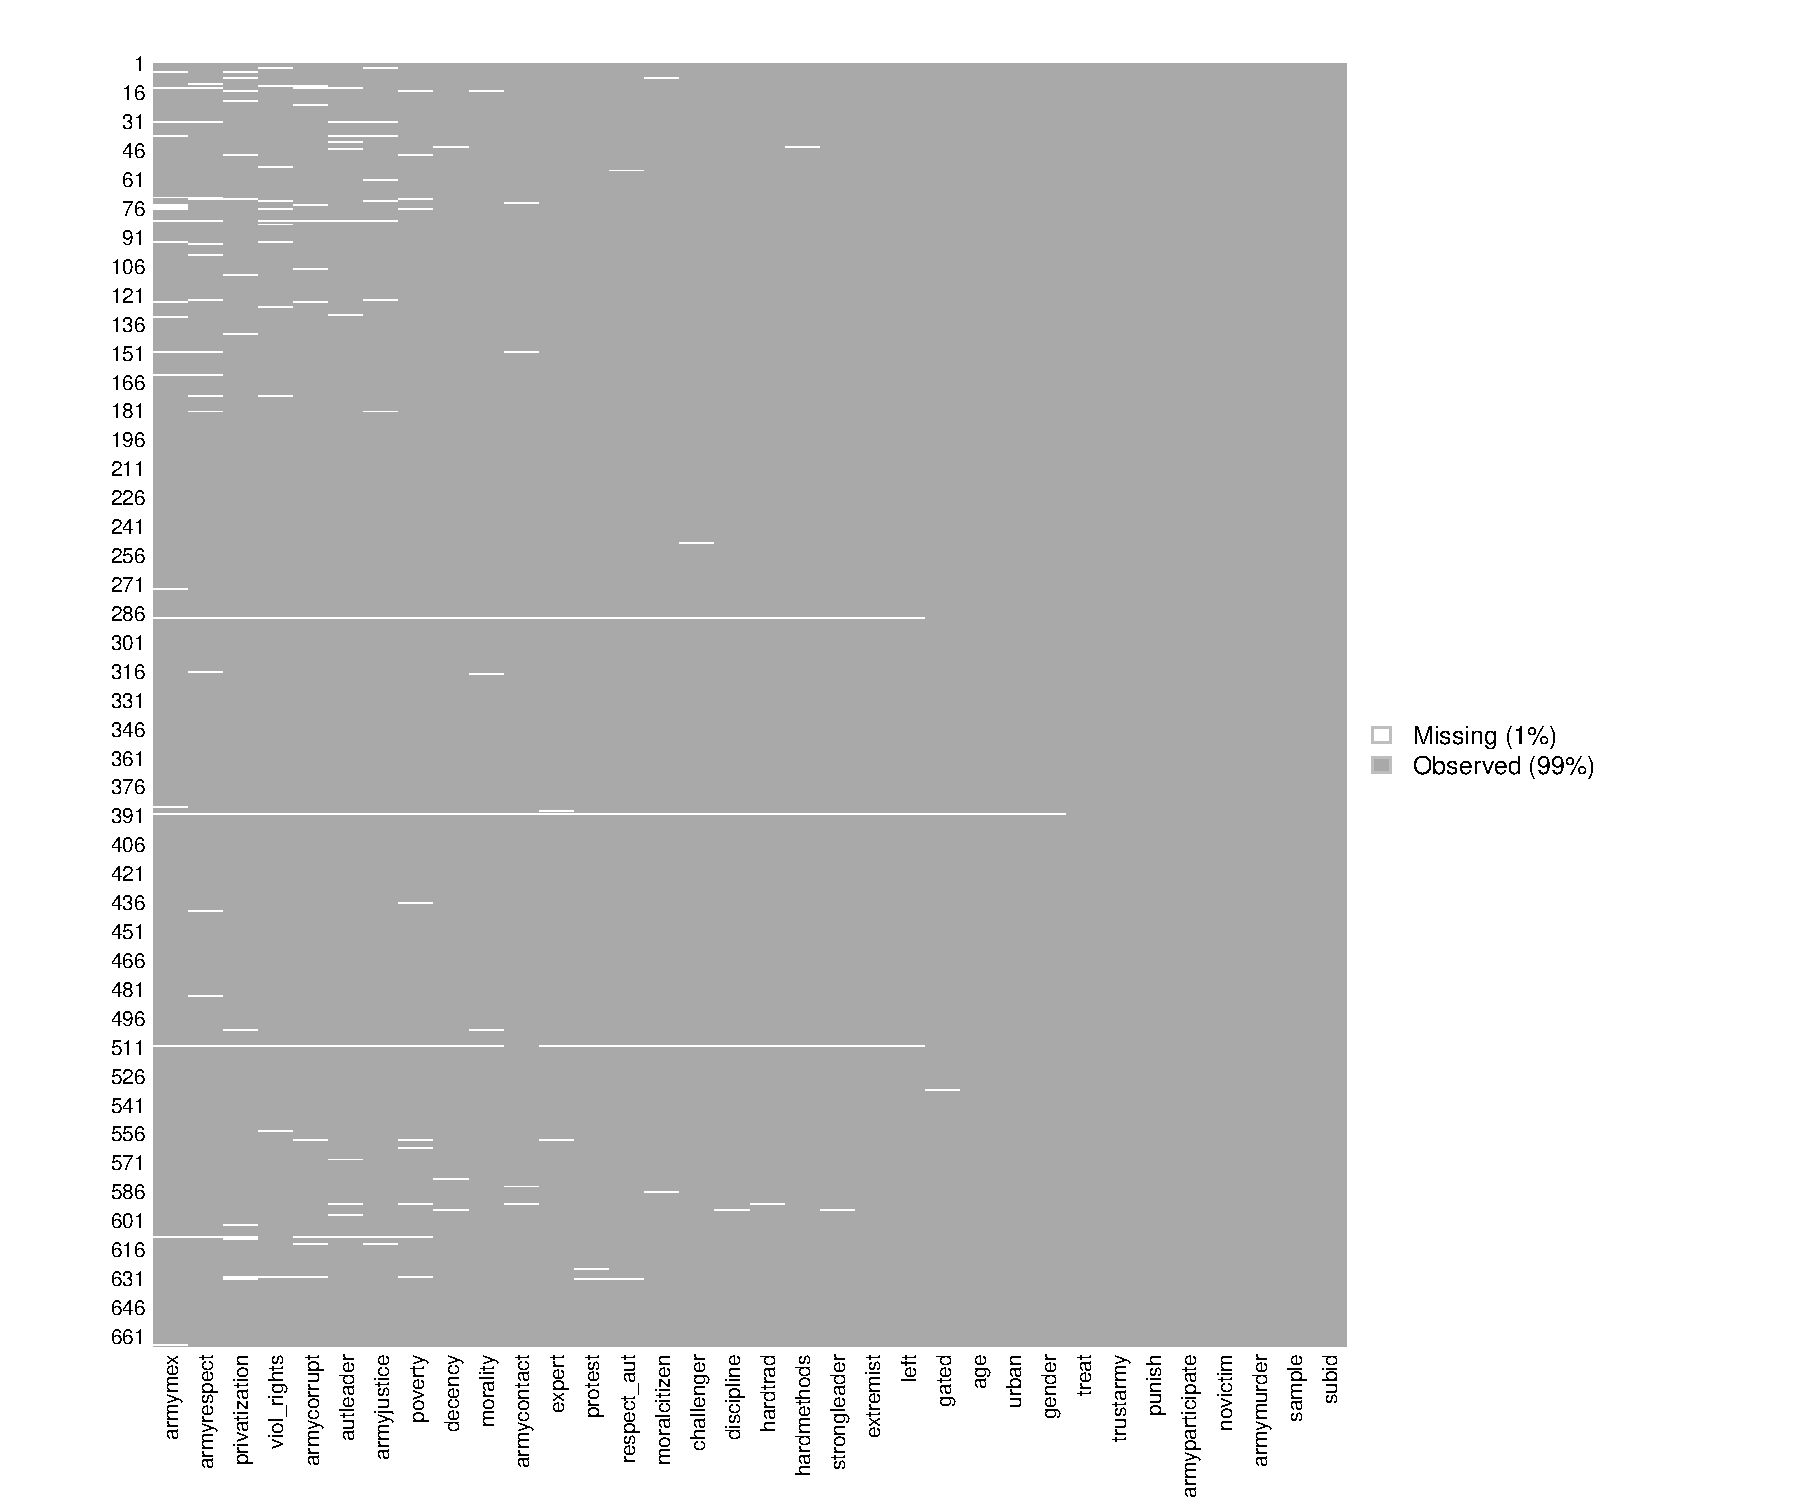
\includegraphics{marko-oliver_final-proj_files/figure-latex/unnamed-chunk-10-1.pdf}
\caption{Missingness Plot}
\end{figure}

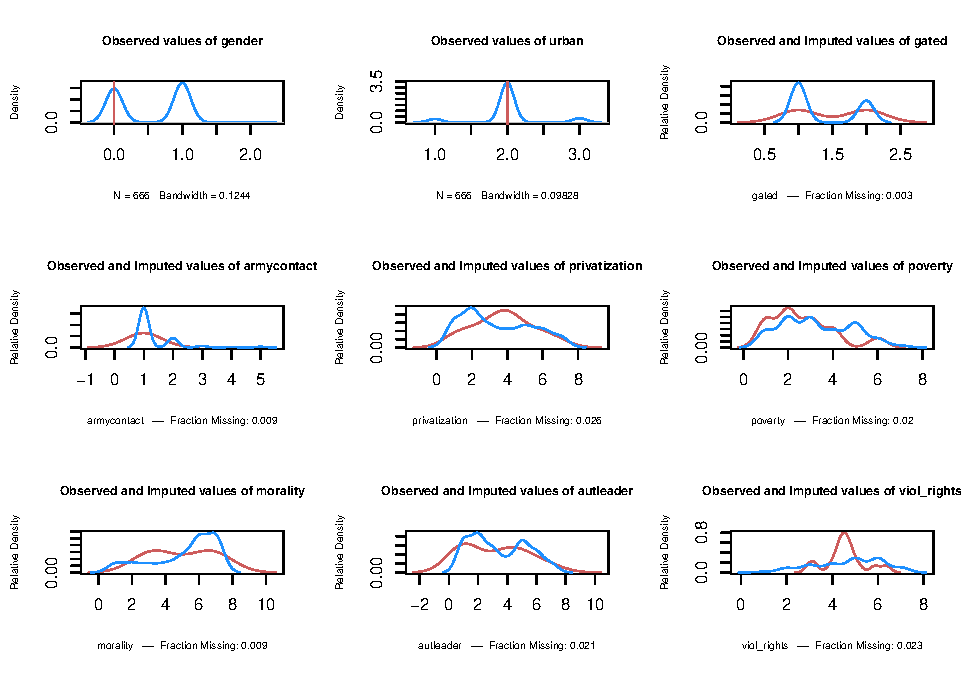
\includegraphics{marko-oliver_final-proj_files/figure-latex/unnamed-chunk-11-1.pdf}
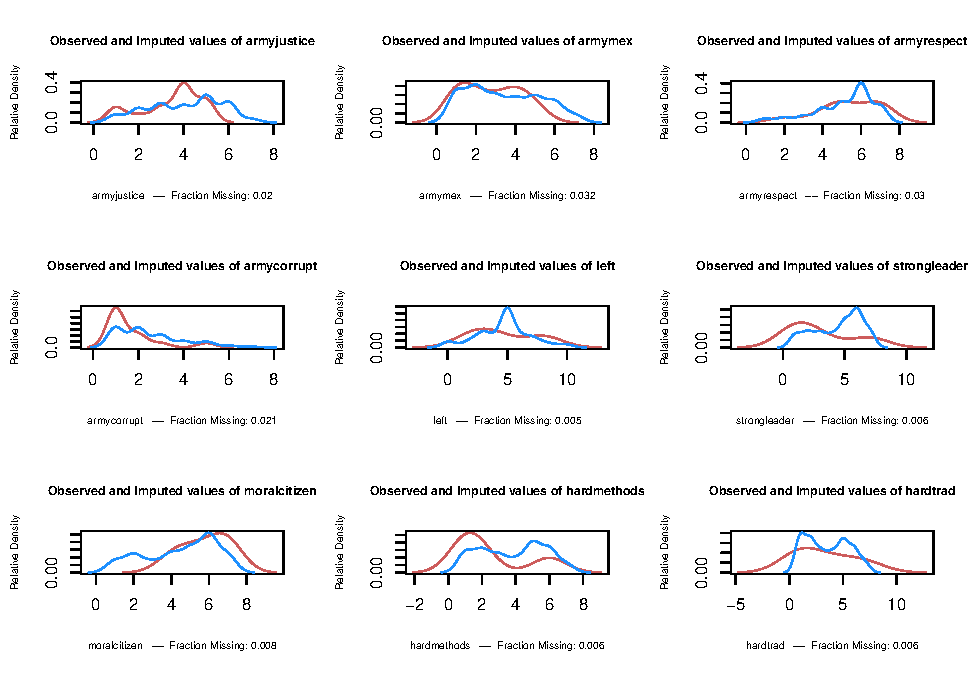
\includegraphics{marko-oliver_final-proj_files/figure-latex/unnamed-chunk-11-2.pdf}
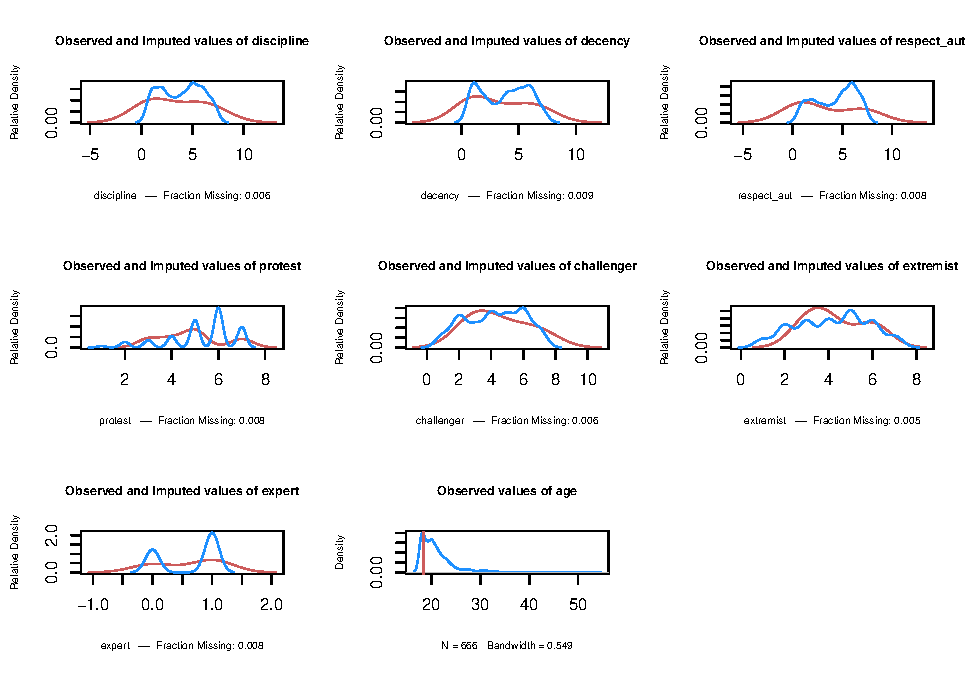
\includegraphics{marko-oliver_final-proj_files/figure-latex/unnamed-chunk-11-3.pdf}

\end{document}
